\documentclass[11pt]{article}
\usepackage[utf8]{inputenc} % Para caracteres en espa�ol
\usepackage{amsmath,amsthm,amsfonts,amssymb,amscd}
\usepackage{multirow,booktabs}
\usepackage[table]{xcolor}
\usepackage{fullpage}
\usepackage{lastpage}
\usepackage{enumitem}
\usepackage{multicol}
\usepackage{fancyhdr}
\usepackage{mathrsfs}
\usepackage{wrapfig}
\usepackage[final]{pdfpages}
\usepackage{setspace}
\usepackage{esvect}
\usepackage{calc}
\usepackage{multicol}
\usepackage{cancel}
\usepackage{graphicx}
\graphicspath{ {pictures/} }
\usepackage[retainorgcmds]{IEEEtrantools}
\usepackage[margin=3cm]{geometry}
\usepackage{amsmath}
\newlength{\tabcont}
\setlength{\parindent}{0.0in}
\setlength{\parskip}{0.05in}
\usepackage{empheq}
\usepackage{framed}
%\usepackage{newtxmath}
\usepackage{euscript}
\DeclareMathAlphabet{\mathpzc}{T1}{pzc}{m}{it}
\usepackage[most]{tcolorbox}
\usepackage{xcolor}
\colorlet{shadecolor}{orange!15}
\parindent 0in
\parskip 12pt
\geometry{margin=1in, headsep=0.25in}
\theoremstyle{definition}
\newtheorem{defn}{Definition}
\newtheorem{reg}{Rule}
\newtheorem{exer}{Exercise}
\newtheorem{note}{Note}
\newcommand{\volume}{{\ooalign{\hfil$V$\hfil\cr\kern0.08em--\hfil\cr}}}
\newcommand{\parr}{\mathbin{\|}} % Parralel Symbol
\begin{document}
\setcounter{section}{5}%Section we want -1
\setcounter{page}{50} %Page we want
\setcounter{equation}{63}%Equation we want -1
\def\thepart{\arabic{part}}
\setcounter{part}{8}
\numberwithin{equation}{part}

 \pagestyle{fancy}
\fancyhf{}
\rhead{Section 8:  Electromagnetic Propulsion - Pulsed Plasma Thruster (PPT)}
\rfoot{Page \thepage}
\thispagestyle{empty}

\begin{center}
{\LARGE \bf Section 8:  Electromagnetic Propulsion}\\
{\large AE435}\\
Spring 2018
\end{center}
\vspace{5mm}
\section{Pulsed Plasma Thruster (PPT)}
\vspace{25mm}
\tableofcontents
\newpage
\subsection{Pulsed Plasma Thruster}
In 1964 Russians decided to avoid problems with tanks, valves, regulators, by using a solid propellant.  The first propellant tried was Teflon, and although many others have been tried, Teflon ($C_2F_4$) remains the best choice.  It has a density almost twice that of Lexan  (2.2 g/cm3).  It does not have a liquid phase, and evaporates from solid to vapor.
 
PPT was first flown in 1964 (Zond 2) and in 1968 (LES-6).  The classic schematic is:
 
 \begin{center}
 \vspace{70mm}
 \textbf{Figure 9: PPT Diagram}
 \end{center}
 %You charge up your capacitor of PFN, you then have an ignitor that creates some seed electrons. We just pulsed that ignotor to create those electrons which will moved to the anode and they will ionize the theflon vapor. We then get an arc that forms across the surface of that teflon which, via jxB pushes the arc out of the chamber. Then you recharge and pulse it again. The surface of the teflon is erroding so the spring pushes the tecflon block till it is depleted. 
 
Parallel plate design.   JxB acceleration.
 
Stored energy is:
  \begin{equation}
\begin{aligned}
\frac{1}{2} C V_o^2 \qquad [J]
\end{aligned}
\end{equation}

For a pulse rate f,  then the average power is

  \begin{equation}
\begin{aligned}
P_{\text{avg}} = f \, E_o \qquad [W]
\end{aligned}
\end{equation}

Typically $f \sim 1-5 Hz$.
 
\newpage Each pulse creates thrust, and evaporates mass, m.
\begin{center}
\vspace{50mm}
 \textbf{Figure 10: Thrust to Propulsion Time}
 \end{center}
We always use bit when talking about pulse devices. The total is over the entire time, the impulse bit is the amount of impulse for one single pulse. Impulse bit is:

  \begin{equation}
\begin{aligned}
\int \, T \, \mathrm{d}t = I_{\text{bit}}
\end{aligned}
\end{equation}
Specific impulse is then:
  \begin{equation}
\begin{aligned}
I_{SP} = \frac{I_{\text{bit}}}{g_o \, m}
\end{aligned}
\end{equation}
 
Average thrust:
   \begin{equation}
\begin{aligned}
\bar{T} \text{ or } T_{\text{avg}} = f \, I_{\text{bit}} \qquad \qquad P_{\text{avg}} = f \, E_o
\end{aligned}
\end{equation}
 
The arc heats the Teflon to $\sim600-700K$, so it ablates.  This ablation continues to occur after the pulsed power is applied. 
 And the ablation that occurs after the initial pulse is referred to as "late time ablation".
 
This is a major source of inefficiency. As we ablate the mass of teflon and when we heat the surface of the teflon, now we have a hot propellant and some of that propellant mass will ablate which is a neutral and slowly drift out of the thruster at a later time. 
   \begin{center}
 \vspace{40mm}
 \textbf{Figure 11: Late Time Ablation Illustration}
 \end{center}
There is no current being forced through the vapor after the mass has be ablated. 
 \newpage
 \subsection{Efficiency}

The efficiency is calculated from a simple circuit model:
\begin{center}
 \vspace{70mm}
 \textbf{Figure 11: Efficiency Circuit Model}
 \end{center}
 
 $Z_o$ is the impedance of the drive circuit, $R_L$ is the load resistance (the joule heating that goes into the heating of the plasma, the switch resistance, the intrinsic PFN resistance), $Z_L$ is the load impedance
 
 
 
Assume a matched PFN: 
   \begin{equation}
\begin{aligned}
R_L + Z_L = Z_o
\end{aligned}
\end{equation}

Thus the voltage drop across the load is equal to that across $Z_o$, that is: $\frac{V_o}{2}$
 
Thus the current is:
    \begin{equation}
\begin{aligned}
J = \frac{\frac{V_o}{2}}{Z_o} = \frac{\frac{V_o}{2}}{R_L + Z_L}
\end{aligned}
\end{equation}
 
Then the charge is:
   \begin{equation*}
\begin{aligned}
Q_o = C_o \, V_o
\end{aligned}
\end{equation*}

And the length of the pulse is

   \begin{equation}
\begin{aligned}
\frac{Q_o}{J} = \frac{C_o \, V_o}{(V_o/2)/Z_o} = 2 \, C_o \, Z_o = t_p
\end{aligned}
\end{equation}
 
Since       $ Z_o = \sqrt{\frac{L}{C}}$               	where L, C are per section of the PFN, and
 
    \begin{equation*}
\begin{aligned}
C_o = N\, C
\end{aligned}
\end{equation*}
Where N is the number of sections in the PFN number. We assume each section has the same capacitance

Then

    \begin{equation}
\begin{aligned}
t_p = 2 \, N \sqrt{L \, C}
\end{aligned}
\end{equation}
 
Recognize that for cases where Electromagnetic energy does work on a mass, thrust in its electromagnetic form is:
 
    \begin{equation*}
\begin{aligned}
\text{Thrust} = F_{em} = \frac{1}{2} \, L' \, J^2
\end{aligned}
\end{equation*}

 and the resulting power
 
    \begin{equation*}
\begin{aligned}
P = \frac{1}{2} \, F \, u_e = J^2 \, Z_o = \frac{1}{2} \bigg( \frac{1}{2} \, L' \, J^2\bigg)\, u_e
\end{aligned}
\end{equation*}

 which means the impedance is
 
    \begin{equation*}
\begin{aligned}
Z_o = \frac{1}{4} \, L' \, u_e
\end{aligned}
\end{equation*}
 
 
 %So if we have a coaxial electrodses, then we will use
Also, for coaxial electrodes, Maecker (8.22) with (8.53) is:
 %Recognizing the electormagnetic thrust is 
 
    \begin{equation*}
\begin{aligned}
F = \frac{\mu \, J^2}{4 \, \pi} \, \bigg(\ln \bigg(\frac{r_a}{r_c}\bigg) + \frac{3}{4}\bigg) = \frac{1}{2} \, L' \, J^2
\end{aligned}
\end{equation*}

   \begin{equation}
\begin{aligned}
L' = \frac{2 \, \mu}{4 \, \pi} \, \bigg(\ln \bigg(\frac{r_a}{r_c}\bigg) + \frac{3}{4}\bigg)
\end{aligned}
\end{equation}
 
 
Returning to efficiency, $R_L$ represents losses in capacitors, switches, electrodes, etc., so let the efficiency:
 
    \begin{equation}
\begin{aligned}
\eta = \frac{Z_L}{R_L + Z_L} = \frac{1}{\frac{R_L}{Z_L}+1}
\end{aligned}
\end{equation}
 Impedance of the load over entire impedance. $R_L$ is the resistive lost in the circuit itself, 
 
 so
    \begin{equation}
\begin{aligned}
Z_L = \frac{1}{4} \, L' \, u_e = \frac{1}{2} \, \frac{\mu}{4 \, \pi} \, \bigg(\ln \bigg(\frac{r_a}{r_c}\bigg) + \frac{3}{4}\bigg) \, u_e
\end{aligned}
\end{equation}

Equation 8.75 is the electromagnetic impedance for coaxial electrodes. The electromagnetic impedance for parallel plate electrodes is somewhere in our notes.

 \begin{framed}
\textbf{For Example:} \\
The resistance $R_L$ is not easy to estimate and is usually done experimentally.

Let $u_e = 2\times10^4 \, m/s$ and our coaxial PPT has the geometry of $\ln(r_a/r_c) + \frac{3}{4} = 2.5$ then we will calculate the $Z_L$ for this thruster to be $Z_L = 2.5 \, m\Omega$, (Equation 8.54)

If resistive losses amounted to $R_L = 5 \, m\Omega$ then we would have an efficiency, $\eta \sim 33 \%$.

Unfortunaly those resistive losses tend to be much higher, around 15 mOhms. 

The advantage of using parallel plate electrodes: recall that $Z = 0.5*k*u_e $ where $k=2.57\times10^{-7}$ for a coaxial geometry and $k \sim 5\times10^{-7}$ for parallel plate geometry. 

Therefore, $Z_L = 5 \, m\Omega$

We would get a little bit higher load impedance meaning we would get a higher efficiency. 
 \end{framed}
 \subsection{Two Stream Model}
 Going back to the idea of late time ablation. At the beginning we have the fast plasma current sheet coming out and then the second phase of slow moving particles coming out.
 
 The first complication is that Teflon ($C_2F_4$) is dissociated to $C+F+F$ and then is partially ionized ($C^+, F^+$).  Because of pressure, neutrals are accelerates to lower velocity than ions.  This leads to a two-stream model.
 
The PPT is partially ionized.  Neutral and Ions.  We have a situation in PPT where the pulse results in "fast" ions and "slow" neutrals coexisting in the same channel.  "Two-Fluid" model.
 
Consider the situation shown here:
 
 \begin{center}
 \vspace{50mm}
 \textbf{Figure 12: Two Fluid Model}
 \end{center}
 \newpage
Total ablated mass is the sum of the fast and slow species.
 
    \begin{equation}
\begin{aligned}
M = M_f + M_s
\end{aligned}
\end{equation}
 
Impulse bit is then:
    \begin{equation}
\begin{aligned}
I_{\text{bit}} = m_f \, u_f + m_s \, u_s
\end{aligned}
\end{equation}
 
Thus $I_{SP}$ and efficiency are:
    \begin{equation}
\begin{aligned}
I_{SP} = \frac{I_{\text{bit}}}{m \, g_o} = \frac{m_f \, u_f + m_s \, u_s}{(m_f + m_s) \, g_o}
\end{aligned}
\end{equation}

    \begin{equation}
\begin{aligned}
\eta = \frac{\frac{1}{2} \, I_{\text{bit}}^2}{m \, E_o}%Just the jet power over total input inergy.
\end{aligned}
\end{equation}

Experimentally we can measure $I_{\text{bit}}$, m and $E_o = \frac{1}{2} \, C \, V_o^2$.  But cannot know $m_f$, $u_f$, $m_s$, $u_s$.  We can also calculate the Electromagnetic portion of $I_{\text{bit}}$:

    \begin{equation}
\begin{aligned}
I_{\text{bit}} = \int \, T_{ET} \, \mathrm{d}t + \int \frac{1}{2}\, L'\, J^2 \, \mathrm{d}t
\end{aligned}
\end{equation}

This total impulse bit is due to two matin things, 1) the electrothermal acceleration of the particles 2) The electromagnetic flow of the thrust, the acceleration of the charged species. This is the total electromagnetic energy deposited in. 
 %
We know geometry, we can measure J so we can evaluate the second integral  

This term is equal to the impulse delivered by the fast species, we can solve for the slow species. 
   \begin{equation}
\begin{aligned}
\int \, \frac{1}{2} \, L' \, J^2 \, \mathrm{d}t = m_f \, u_f
\end{aligned}
\end{equation}

Then from measured $I_{\text{bit}}$, we also know $m_s u_s$; solve Equation 8.80 for 

    \begin{equation*}
\begin{aligned}
\int \, T_{ET} \, \mathrm{d}t = m_s u_s
\end{aligned}
\end{equation*}
 
Now the problem is, what are $m_f$ and $m_s$, or $u_f$ and $u_s$?

We don't know how much of our mass is the fast species and how much is the slow species.

We find the answer in Cosmology, more specifically a theory for the origin of the solar system by Hannes Alfven (Nobel Prize in Physics 1970).  Alfven's paper "On the Origin of the Solar System" assumed the Sun and a magnetized dust cloud.
 
 
 
 %The critical velo
 
 
 
 
 
Alfven: When KE = ionization energy, particle falling in is ionized, losing all energy, so stops.  In this way, atoms of H, He, Ne, etc. stop at different radii.
 
    \begin{equation}
\begin{aligned}
\frac{1}{2} \, m \, u_c^2 = e \, \varepsilon_i
\end{aligned}
\end{equation}
 
So for the PPT it is assumed that $u_f$ cannot exceed $u_s$ by more than $u_c$:
 
 If we have this mass of slow species moving along, then the ions cannot leave faster than this critical speed. Whenever the KE = Ionization, the particles transfers all of its KE to Ionization energy and no longer moves, generally caused by collisions. 
 
    \begin{equation}
\begin{aligned}
u_f - u_s = u_c
\end{aligned}
\end{equation}
 
What is $u_c$ for Teflon (CF$_2$)?%What would tehrse values be for teflon that we are wokring with. 

Critical velocity for Carbon: $u_c = 13 \, [km/s]$

Critical velocity for Fluorine: $u_c = 13 \, [km/s]$
\begin{framed}
Example, assume the net exit velocity is $10.5 \, km/s$ due to both $m_s$ and $m_f$. 
\vspace{70mm}
 \end{framed}
 
 
 
Conclusion:  Most efficient PPT has highest degree of ionization, which minimizes ms and raises Isp.
 
 



  \newpage
 \subsection{More Advanced PPT Modeling}
More advanced PPT models use an ablation model
connected with an electrothermal or electromagnetic (i.e.,
electromechanical) acceleration model connected with a
plume model.

\subsubsection{Ablation Model:}
\begin{center}
{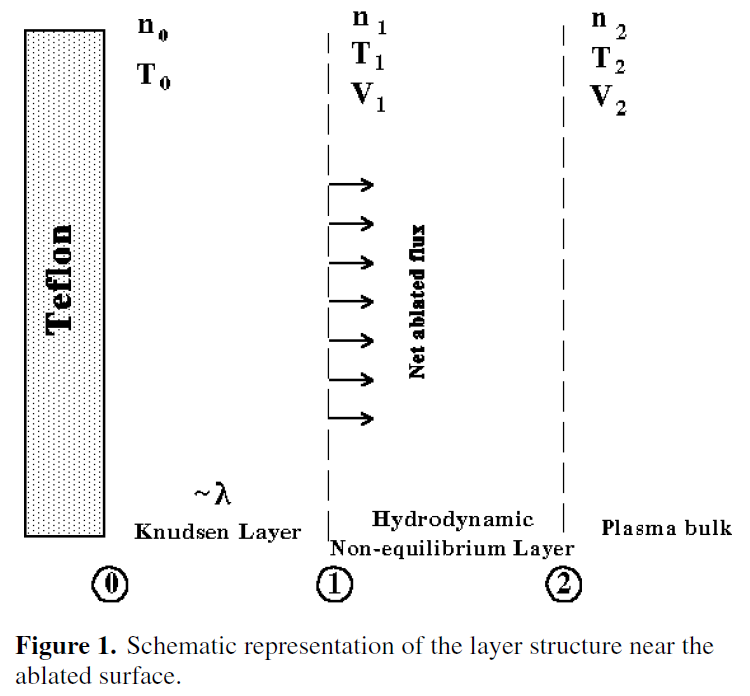
\includegraphics[scale=0.5]{f1.png}}
\end{center}
Non-equilibrium kinetic layer near the surface of ablating
material. Two extremes are the surface and the plasma
bulk. In between one can imagine a kinetic non-equilibrium
layer close to the surface with a thickness a
few mean free paths (Knudsen layer). Then a collision dominated
non-equilibrium layer where electron and
heavy particle temperatures differ. At the right, all
species reach thermal equilibrium.

Michael, K., Iain, D. B., Isak, I. B., "On the model of
Teflon ablation in an ablation-controlled discharge,"
Journal of Physics D: Applied Physics, Vol. 34, No. 11,
pp. 1675, 2001.

\subsubsection{Electrothermal Model}
\begin{center}
{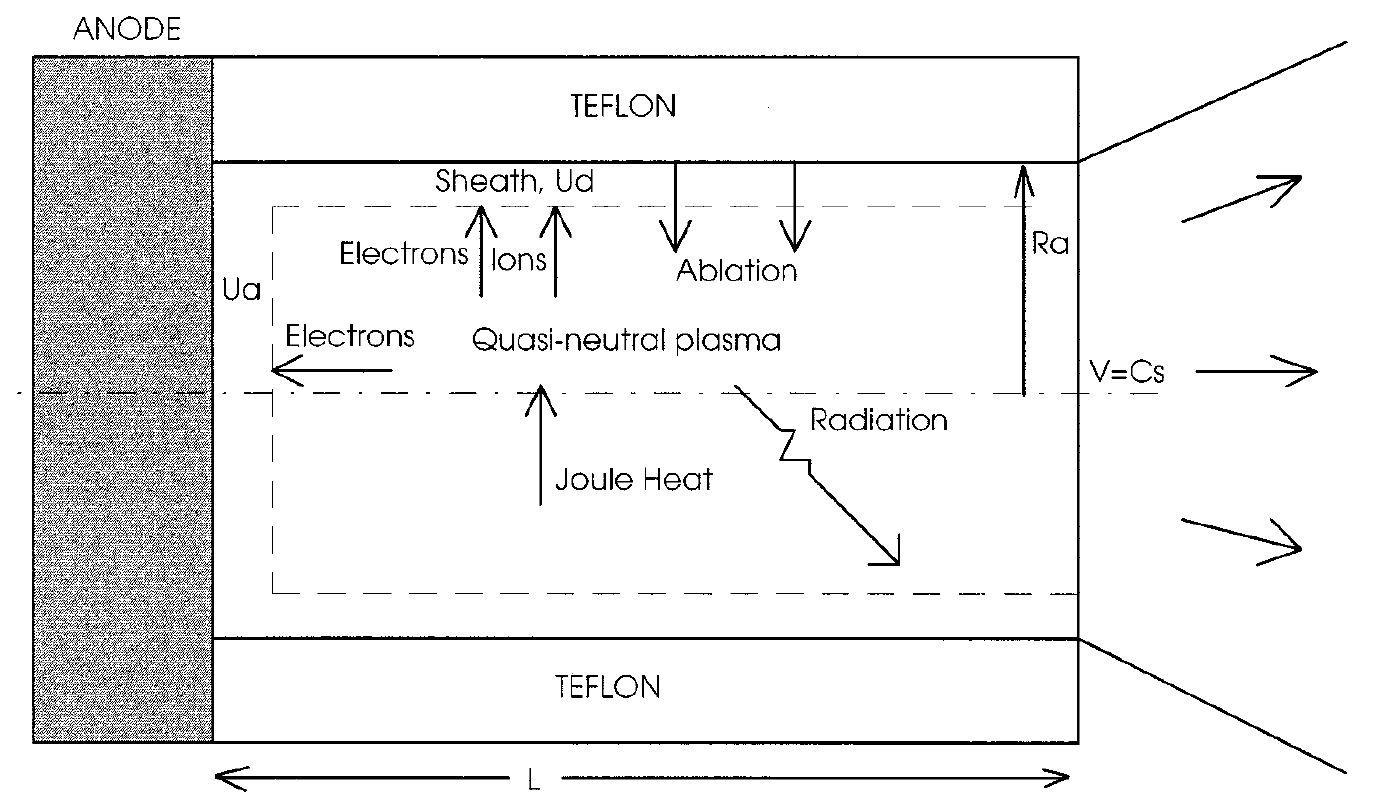
\includegraphics[scale=0.4]{f2.png}}
\end{center}
Plasma heating with electrothermal acceleration.
Energy balance in the quasineutral plasma column is:

Keidar, M., Boyd, I. D., Beilis, I. I., "Electrical discharge
in the Teflon cavity of a coaxial pulsed plasma thruster,"
Plasma Science, IEEE Transactions on, Vol. 28, No. 2,
pp. 376-385, 2000

\subsubsection{Electromagnetic Model with Plume}
\begin{center}
{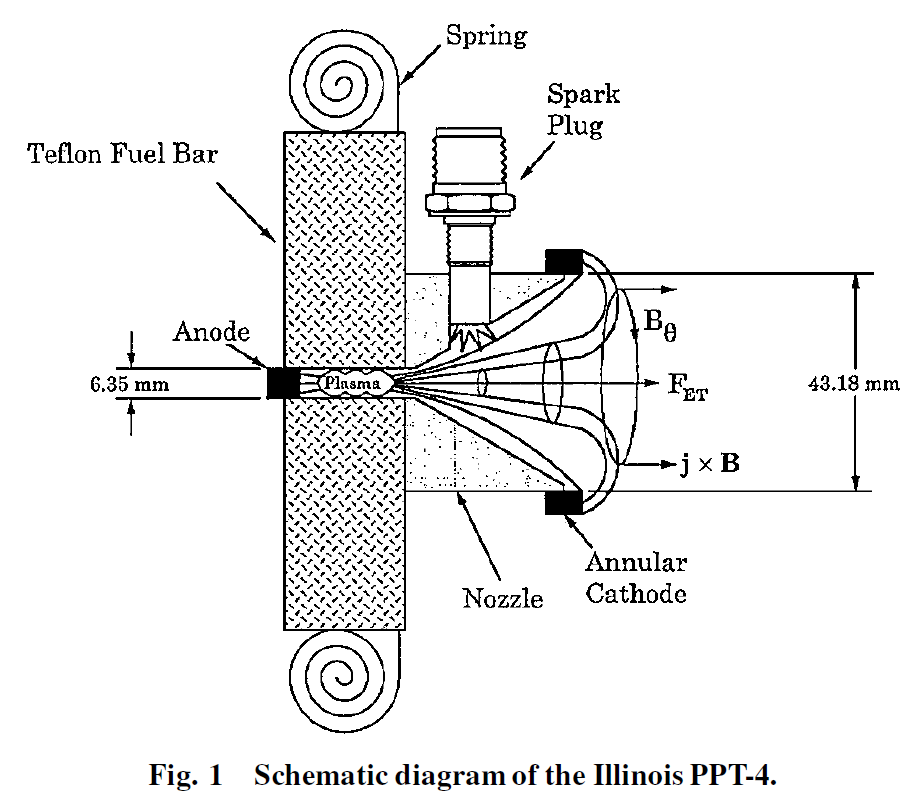
\includegraphics[scale=0.5]{f3.png}}
\end{center}
Boyd, I. D., Keidar, M., McKeon, W., "Modeling of a
Pulsed Plasma Thruster from Plasma Generation to Plume
Far Field," Journal of Spacecraft and Rockets, Vol. 37,
No. 3, pp. 399-407, 2000/05/01.
%Breaking up PPT into phases (ablation, discharge model/electrothemra/magneticl model)
%Start with ana ablation model like the the (heat of vaporiation, )

\end{document}